% Gabarit pandoc des corrigés publiés (brut et guidé). Contenu sans marque ni nom de site.
% Compilation : lualatex (latexmk -lualatex).
% Le Markdown reste la source unique : ne pas éditer ce fichier .tex à la main.
\documentclass[11pt,a4paper]{article}

% --- Moteur, polices (Latin Modern) et langue ---------------------------------
\usepackage{iftex}
\ifLuaTeX\else\errmessage{Ce document se compile avec lualatex}\fi
\usepackage{amsmath,amssymb,mathtools}
\usepackage{fontspec}
% mathrm=sym : \mathrm prend ses glyphes dans la police mathématique (ℓ, μ, Ω), comme KaTeX.
\usepackage[math-style=TeX,bold-style=TeX,mathrm=sym]{unicode-math}
% Repli pour les glyphes absents de Latin Modern (indices et exposants Unicode,
% flèches, filets des schémas en texte, symboles) : DejaVu, puis Latin Modern Math
% (ℓ, lettres mathématiques Unicode des légendes).
\directlua{
  luaotfload.add_fallback("repliTexte", {"DejaVuSerif:mode=harf;", "DejaVuSans:mode=harf;", "file:latinmodern-math.otf:mode=harf;"})
  luaotfload.add_fallback("repliMono", {"DejaVuSansMono:mode=harf;", "DejaVuSans:mode=harf;", "file:latinmodern-math.otf:mode=harf;"})
}
\setmainfont{Latin Modern Roman}[RawFeature={fallback=repliTexte}]
\setsansfont{Latin Modern Sans}[RawFeature={fallback=repliTexte}]
\setmonofont{Latin Modern Mono}[RawFeature={fallback=repliMono}]
\setmathfont{Latin Modern Math}
\usepackage[french]{babel}
\frenchsetup{SmallCapsFigTabCaptions=false}

% --- Mise en page --------------------------------------------------------------
\usepackage[a4paper,margin=2.2cm,headheight=14pt,footskip=1.2cm]{geometry}
\usepackage{microtype}
\setlength{\emergencystretch}{4em}
\tolerance=1500
\setlength{\parindent}{0pt}
\setlength{\parskip}{0.55\baselineskip plus 2pt minus 1pt}
\usepackage{xcolor}
% Gris nommés : babel-french rend « ! » actif dans le document.
\definecolor{gris2}{gray}{0.98}
\definecolor{gris3}{gray}{0.97}
\definecolor{gris5}{gray}{0.95}
\definecolor{gris35}{gray}{0.65}
\definecolor{gris40}{gray}{0.60}
\definecolor{gris45}{gray}{0.55}
\definecolor{gris50}{gray}{0.50}
\definecolor{gris55}{gray}{0.45}
\definecolor{gris60}{gray}{0.40}
\definecolor{gris65}{gray}{0.35}
\definecolor{gris70}{gray}{0.30}
\definecolor{gris80}{gray}{0.20}
\definecolor{gris85}{gray}{0.15}
\usepackage{graphicx}
\usepackage{float}
\usepackage{caption}
\captionsetup{font=small,labelformat=empty,justification=centering}
\usepackage{booktabs,longtable,array,multirow,calc}
\usepackage{siunitx}
\sisetup{locale=FR}
\usepackage[version=4]{mhchem}
\usepackage{listings}
\usepackage{fancyhdr}
\usepackage{lastpage}
\usepackage[most]{tcolorbox}
\usepackage{enumitem}
\setlist{nosep,leftmargin=*,topsep=2pt}
\usepackage[hidelinks,unicode]{hyperref}
\usepackage{bookmark}
\hypersetup{pdftitle={Mines-Ponts PSI — Maths 2 2026},pdfauthor={Rédigé par IA},pdfcreator={LaTeX},pdfsubject={Corrigé guidé}}
\usepackage{xurl}

% --- Pandoc : listes, tableaux, figures ----------------------------------------
\providecommand{\passthrough}[1]{#1}
\providecommand{\tightlist}{\setlength{\itemsep}{0pt}\setlength{\parskip}{0pt}}

\makeatletter
\def\maxwidth{\ifdim\Gin@nat@width>\linewidth\linewidth\else\Gin@nat@width\fi}
\def\maxheight{\ifdim\Gin@nat@height>0.55\textheight 0.55\textheight\else\Gin@nat@height\fi}
\makeatother
\setkeys{Gin}{width=\maxwidth,height=\maxheight,keepaspectratio}
\setcounter{secnumdepth}{-\maxdimen}
\providecommand{\pandocbounded}[1]{#1}

% --- Code (listings) -----------------------------------------------------------
\lstset{
  basicstyle=\ttfamily\small,
  columns=fullflexible,
  keepspaces=true,
  breaklines=true,
  breakatwhitespace=false,
  postbreak=\mbox{\textcolor{gris50}{$\hookrightarrow$}\space},
  frame=single,
  rulecolor=\color{gris35},
  framesep=4pt,
  xleftmargin=5pt,xrightmargin=5pt,
  backgroundcolor=\color{gris3},
  keywordstyle=\bfseries,
  commentstyle=\color{gris65},
  stringstyle=\color{gris80},
  showstringspaces=false,
  tabsize=4,
  extendedchars=true,
  aboveskip=6pt,belowskip=6pt,
}

% --- Macros des corrigés (KaTeX ↔ LaTeX) ---------------------------------------
% Les corrigés sont écrits pour KaTeX : on définit ici ce que KaTeX connaît et
% que LaTeX n'a pas, sans jamais retoucher le Markdown.
\providecommand{\R}{\mathbb{R}}
\providecommand{\N}{\mathbb{N}}
\providecommand{\Z}{\mathbb{Z}}
\providecommand{\Q}{\mathbb{Q}}
\providecommand{\C}{\mathbb{C}}
\providecommand{\dd}{\mathrm{d}}
\providecommand{\llbracket}{\lBrack}
\providecommand{\rrbracket}{\rBrack}
\providecommand{\lBrace}{\lbrace}
\providecommand{\rBrace}{\rbrace}
\providecommand{\Box}{\square}
\providecommand{\Diamond}{\lozenge}
\providecommand{\varnothing}{\emptyset}
\providecommand{\argmax}{\operatorname*{arg\,max}}
\providecommand{\argmin}{\operatorname*{arg\,min}}
\renewcommand{\leq}{\leqslant}
\renewcommand{\geq}{\geqslant}

% Équation hors texte : réduite à la largeur de la ligne si elle déborde.
\newsavebox{\boiteequation}
\newcommand{\equationajustee}[1]{%
  \sbox{\boiteequation}{$\displaystyle #1$}%
  \ifdim\wd\boiteequation>\linewidth
    \[\resizebox{\linewidth}{!}{\usebox{\boiteequation}}\]%
  \else
    \[#1\]%
  \fi}

% --- Encadrés pédagogiques (sobres, lisibles en noir et blanc) -----------------
\tcbset{
  encadre/.style={
    enhanced,breakable,sharp corners,
    colback=white,colframe=gris55,
    boxrule=0.4pt,leftrule=2.2pt,
    left=6pt,right=6pt,top=3pt,bottom=3pt,
    before skip=6pt,after skip=6pt,
    fonttitle=\bfseries\small,coltitle=black,
    attach title to upper,after title={\quad},
    parbox=false,
  }
}
\newtcolorbox{indication}[1]{encadre,colframe=gris45,colback=gris2,title={Indication~#1}}
\newtcolorbox{methode}{encadre,colframe=gris70,title={Méthode}}
\newtcolorbox{piege}{encadre,colframe=gris85,boxrule=0.8pt,leftrule=2.2pt,title={Piège}}
\newtcolorbox{jury}{encadre,colframe=gris60,colback=gris5,title={Jury}}
\newtcolorbox{encadrenote}{encadre,colframe=gris40}

% --- Titres de section ---------------------------------------------------------
\usepackage{titlesec}
\titleformat{\section}{\Large\bfseries}{}{0pt}{}
\titleformat{\subsection}{\large\bfseries}{}{0pt}{}
\titleformat{\subsubsection}{\normalsize\bfseries}{}{0pt}{}
\titlespacing*{\section}{0pt}{14pt plus 4pt minus 2pt}{6pt}
\titlespacing*{\subsection}{0pt}{10pt plus 3pt minus 2pt}{4pt}
\titlespacing*{\subsubsection}{0pt}{8pt plus 2pt minus 2pt}{2pt}

% --- En-tête et pied de page ---------------------------------------------------
\pagestyle{fancy}
\fancyhf{}
\fancyhead[L]{\small\textsc{Corrigé guidé} · Mines-Ponts PSI}
\fancyhead[R]{\small Maths 2 2026}
\fancyfoot[L]{\footnotesize Corrigé rédigé par IA, non officiel}
\fancyfoot[R]{\footnotesize \thepage\,/\,\pageref*{LastPage}}
\renewcommand{\headrulewidth}{0.4pt}
\renewcommand{\footrulewidth}{0pt}
\fancypagestyle{plain}{\fancyhf{}\fancyfoot[R]{\footnotesize \thepage\,/\,\pageref*{LastPage}}\fancyfoot[L]{\footnotesize Corrigé rédigé par IA, non officiel}\renewcommand{\headrulewidth}{0pt}}

\begin{document}
\thispagestyle{plain}
\begin{center}
  {\small\scshape Corrigé guidé}\par\smallskip
  {\LARGE\bfseries Mines-Ponts PSI — Maths 2 2026\par}\medskip
  {\large Mines-Ponts · PSI · Maths 2 · 2026\par}
\end{center}
\vspace{2pt}\hrule\vspace{8pt}

\emph{Corrigé rédigé par IA, non officiel. Signalez toute erreur.}

\hypertarget{pruxe9sentation-du-sujet}{%
\section{Présentation du sujet}\label{pruxe9sentation-du-sujet}}

\textbf{Thème.} Le problème calcule la probabilité \(q_n(k)\) qu'un entier tiré uniformément dans \([\![1;n]\!]\) soit \emph{sans facteur à la puissance \(k\)} : aucun \(p^k\), \(p\) premier, ne le divise. Il montre que \(q_n(k)\to\frac1{\zeta(k)}\).

En chemin, il démontre les formules d'Euler \(\zeta(2)=\frac{\pi^2}{6}\) et \(\zeta(4)=\frac{\pi^4}{90}\), si bien que la conclusion est explicite : un entier « au hasard » est sans facteur carré avec probabilité \(\frac{6}{\pi^2}\approx0{,}61\).

\textbf{Découpage (25 questions, 3 heures, sans calculatrice ni document).}

\begin{itemize}
\tightlist
\item
  \textbf{Partie 1 (Q1--Q9), calcul de \(\sum\frac1{n^2+x^2}\).} On obtient \(\sum_{k\ge1}\frac{\sin(k\theta)}{k}=\frac{\pi-\theta}{2}\), puis l'expression de \(S(t)=\sum\frac{\cos(nt)}{n^2}\) sur \([0;\pi]\). On étudie ensuite \(g_x(t)=\sum\frac{\cos(nt)}{n^2(n^2+x^2)}\), solution d'une équation différentielle à coefficients constants. Son calcul explicite donne \(\frac{2\pi x}{e^{2\pi x}-1}=1-\pi x+\sum\frac{2x^2}{n^2+x^2}\).
\item
  \textbf{Partie 2 (Q10--Q14), développement de \(h(x)=\frac{x}{e^x-1}\).} Somme géométrique finie, contrôle du reste, changement de variable \(X=2\pi x\), produit de Cauchy : on obtient les coefficients \(b_k\) (nombres de Bernoulli), puis \(\zeta(2)\) et \(\zeta(4)\).
\item
  \textbf{Partie 3 (Q15--Q20), dénombrement.} Développement d'un produit, formule du crible démontrée par les indicatrices, fonction de Möbius. On obtient \(q_n(k)=\frac1n\sum_d\mu(d)\lfloor n/d^k\rfloor\), puis on passe à la limite par convergence dominée.
\item
  \textbf{Partie 4 (Q21--Q25), identité \(\sum\mu(i)i^{-s}=\frac1{\zeta(s)}\).} Produit de deux séries traité « à la main » par un encadrement entre un carré et des régions sous des hyperboles, puis la propriété \(\sum_{d\mid m}\mu(d)=[m=1]\).
\end{itemize}

Les parties 1--2 et 3--4 forment deux blocs indépendants ; seules Q9 (pour la partie 2) et Q14 (pour Q25) font le pont. Le programme de PSI ne donne le théorème de Fubini et la sommation par paquets que dans le cadre des familles sommables, « strictement réservé au contexte probabiliste » ; hors probabilités, ils ne sont pas disponibles pour les sommes doubles : le rapport 2026 explique qu'une bonne partie des questions des parties 2 et 4 sont des voies de contournement élémentaires de ces théorèmes.

\textbf{Notions mobilisées.} Sommes géométriques ; intégrales sur un segment ; séries numériques et de fonctions (convergence normale, uniforme, continuité, intégration et dérivation terme à terme) ; équations différentielles linéaires d'ordre 2 à coefficients constants ; séries entières (rayon, produit de Cauchy, unicité des coefficients) ; espérance et indicatrices ; théorème de convergence dominée ; arithmétique élémentaire.

\textbf{Ce qu'en dit le rapport 2026.} La partie 1, technique, a « cueilli les candidats à froid » : ils ne se sont mis en valeur que sur Q1, le début de Q3, Q4, Q6, les calculs de Q7 et la conclusion Q9. La partie 2 a été mieux réussie. Beaucoup de candidats se sont arrêtés là ; ceux qui ont abordé les probabilités ont surtout traité Q15 à Q18, et le début de Q21.

\textbf{Questions abordables à ne pas laisser passer.} Q1, Q4, Q6, Q7, Q9 (purement algébrique si l'on admet Q8), Q10, Q14 (calculable en admettant Q12--Q13), Q15, Q16, Q17, les inclusions de Q21, Q23, Q24, Q25 (rédigeable en admettant Q20 et Q24).

\textbf{Questions discriminantes}, d'après le rapport 2026 :

\begin{itemize}
\tightlist
\item
  Q5, « fort délicate », presque jamais résolue ;
\item
  Q8, résolution complète de l'équation différentielle, très mal réussie ;
\item
  le début de Q11, qui a mis en valeur ceux qui maîtrisent les théorèmes sur les séries de fonctions ;
\item
  le calcul de \(b_4\) et \(\zeta(4)\) en Q14, rarement abouti ;
\item
  Q19, presque jamais résolue, et Q20, dont le lien avec la convergence dominée n'a pas été vu.
\end{itemize}

\textbf{Gestion du temps.} Sujet long mais très guidé. Le rapport 2026 rappelle : « Beaucoup de candidats ont réussi à avoir une note décente en ne traitant correctement que 6 ou 7 questions. » Mieux vaut des questions faciles complètement justifiées que du picorage en fin de sujet.

\hypertarget{partie-1-calcul-de-la-somme-sum_n1inftyfrac1n2x2}{%
\section{\texorpdfstring{Partie 1 --- Calcul de la somme \(\sum_{n=1}^{+\infty}\frac{1}{n^2+x^2}\)}{Partie 1 --- Calcul de la somme \textbackslash sum\_\{n=1\}\^{}\{+\textbackslash infty\}\textbackslash frac\{1\}\{n\^{}2+x\^{}2\}}}\label{partie-1-calcul-de-la-somme-sum_n1inftyfrac1n2x2}}

On part de la série \(\sum e^{ik\theta}/k\), qu'on écrit comme une intégrale ; sa partie imaginaire donne \(\sum\sin(k\theta)/k\), que l'on intègre pour obtenir \(S\).

Ensuite \(g_x\) vérifie une équation différentielle dont le second membre, grâce à \(S\), est polynomial sur \([0;\pi]\). On la résout et on lit \(g_x''(0)=-\sum\frac{1}{n^2+x^2}\).

\hypertarget{question-1}{%
\subsection{Question 1}\label{question-1}}

\begin{indication}{1}

Le quotient \(\frac{1-(e^{i\theta}t)^n}{1-e^{i\theta}t}\) doit vous rappeler une formule bien connue.

\end{indication}

\begin{indication}{2}

Avant tout calcul, vérifiez que l'intégrale de l'énoncé a un sens : le dénominateur peut-il s'annuler sur \([0;1]\) ? Puis développez et intégrez une somme finie.

\end{indication}

\hypertarget{solution}{%
\subsubsection{Solution}\label{solution}}

Soit \(\theta\in\mathbb{R}\setminus2\pi\mathbb{Z}\) et \(n\in{\mathbb{N}}^*\). Pour \(t\in[0;1]\), on a \(|e^{i\theta}t|=t\le1\).

Si l'on avait \(e^{i\theta}t=1\), on aurait \(t=|e^{i\theta}t|=1\), puis \(e^{i\theta}=1\), soit \(\theta\in2\pi\mathbb{Z}\) : c'est exclu.

Le dénominateur ne s'annule donc pas, et l'intégrande est continue sur \([0;1]\).

La raison \(e^{i\theta}t\) étant différente de \(1\), la somme géométrique finie donne
\equationajustee{\begin{aligned}
e^{i\theta}\,\frac{1-(e^{i\theta}t)^n}{1-e^{i\theta}t}&=e^{i\theta}\sum_{j=0}^{n-1}(e^{i\theta}t)^j\\
&=\sum_{k=1}^{n}e^{ik\theta}t^{k-1}.
\end{aligned}}
On intègre par linéarité de l'intégrale sur une somme \textbf{finie}, avec \(\int_0^1t^{k-1}\,\mathrm{d}t=\frac1k\) :
\equationajustee{\boxed{\int_0^1e^{i\theta}\,\frac{1-(e^{i\theta}t)^n}{1-e^{i\theta}t}\,\mathrm{d}t=\sum_{k=1}^{n}\frac{e^{ik\theta}}{k}.}}

\begin{methode}

Pour écrire une somme \(\sum a_k/k\) comme une intégrale, on remplace \(\frac1k\) par \(\int_0^1t^{k-1}\,\mathrm{d}t\) et on somme sous l'intégrale. Sur une somme finie, aucune hypothèse n'est requise ; c'est le passage à la limite qui demandera du travail.

\end{methode}

\begin{jury}

Le rapport 2026 note que « Trop peu de candidats ont pris la peine de vérifier que la raison diffère bien de 1 lorsque \(t\) parcourt l'intervalle indiqué », et que presque personne ne l'a déduit précisément de \(\theta\notin2\pi\mathbb{Z}\). Il relève aussi des bornes fausses dans la formule de sommation géométrique, rattrapées ensuite par un tour de passe-passe que les correcteurs détectent.

\end{jury}

\hypertarget{question-2}{%
\subsection{Question 2}\label{question-2}}

\begin{indication}{1}

Écrivez la différence entre la somme partielle et l'intégrale limite comme une seule intégrale, et majorez-la.

\end{indication}

\begin{indication}{2}

Il faut minorer \(|1-e^{i\theta}t|\) par une constante strictement positive indépendante de \(t\in[0;1]\). Calculez son carré et faites apparaître une somme de deux carrés.

\end{indication}

\hypertarget{solution-1}{%
\subsubsection{Solution}\label{solution-1}}

\textbf{Minoration du dénominateur.} Pour \(u\in[0;1]\),
\equationajustee{\begin{aligned}
|1-e^{i\theta}u|^2&=1-2u\cos\theta+u^2\\
&=(u-\cos\theta)^2+\sin^2\theta.
\end{aligned}}
Si \(\sin\theta\ne0\), on en tire \(|1-e^{i\theta}u|\ge|\sin\theta|\).

Si \(\sin\theta=0\), comme \(\theta\notin2\pi\mathbb{Z}\), on a \(\cos\theta=-1\), d'où \(|1-e^{i\theta}u|=1+u\ge1\).

Avec \(c_\theta=\min(1,|\sin\theta|)>0\), on obtient dans tous les cas
\equationajustee{(\star)\qquad\forall u\in[0;1],\ |1-e^{i\theta}u|\ge c_\theta.}

\begin{figure}[H]
\centering
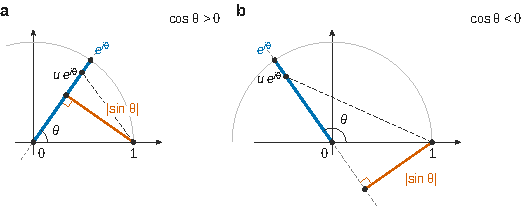
\includegraphics{figures/q2-distance-segment.pdf}
\caption*{Figure 1 --- Distance du point 1 au segment d'extrémités 0 et
e\^{}\{iθ\} : elle est au moins \textbar sin θ\textbar, distance de 1 à
la droite portant le segment, que le pied de la perpendiculaire soit sur
le segment (a) ou sur son prolongement (b)}
\end{figure}

\textbf{Convergence.} Notons \(I(\theta)=\int_0^1\frac{e^{i\theta}}{1-e^{i\theta}t}\,\mathrm{d}t\) (intégrande continue d'après \((\star)\)). Par la question 1,
\equationajustee{\sum_{k=1}^{n}\frac{e^{ik\theta}}{k}-I(\theta)=-\int_0^1\frac{e^{i\theta}(e^{i\theta}t)^n}{1-e^{i\theta}t}\,\mathrm{d}t.}
On majore le module de l'intégrale par l'intégrale du module, puis on utilise \((\star)\) :
\equationajustee{(\star\star)\qquad\begin{aligned}
\left|\sum_{k=1}^{n}\frac{e^{ik\theta}}{k}-I(\theta)\right|&\le\int_0^1\frac{t^n}{c_\theta}\,\mathrm{d}t\\
&=\frac{1}{c_\theta(n+1)}.
\end{aligned}}
Ce majorant tend vers \(0\) quand \(n\to+\infty\). \textbf{La série \(\sum_{k\ge1}\frac{e^{ik\theta}}{k}\) converge} et
\equationajustee{\boxed{\sum_{k=1}^{+\infty}\frac{e^{ik\theta}}{k}=\int_0^1\frac{e^{i\theta}}{1-e^{i\theta}t}\,\mathrm{d}t.}}

\begin{piege}

Toute inégalité porte sur des réels : on majore des \textbf{modules}, jamais des nombres complexes. Le rapport 2026 est net : « La plupart des erreurs sont provenues de tentatives de majorations de nombres complexes, ce qui a été justement (donc lourdement) sanctionné. » Minorer \(|1-e^{i\theta}t|\) par \(1-t\) ne mène à rien non plus : ce minorant s'annule en \(t=1\).

\end{piege}

\begin{jury}

Le rapport 2026 indique comme voie la plus courte la convergence dominée, à mener sur \([0;1[\) (la convergence simple n'a pas lieu en \(1\)), avec une fonction dominante dont l'intégrabilité se justifie par prolongement continu à \([0;1]\). La majoration directe \((\star\star)\) ci-dessus évite ce théorème et fournit en prime une estimation uniforme utile en question 5.

\end{jury}

\begin{methode}

Gardez en tête que la majoration \((\star\star)\) est \textbf{uniforme} en \(\theta\) dès que \(|\sin\theta|\) est minoré : c'est l'outil qui débloque la question 5.

\end{methode}

\hypertarget{question-3}{%
\subsection{Question 3}\label{question-3}}

\begin{indication}{1}

Prenez la partie imaginaire du résultat de la question 2, en justifiant le passage à la partie imaginaire d'une série convergente.

\end{indication}

\begin{indication}{2}

Pour la partie imaginaire de l'intégrande, multipliez par le conjugué du dénominateur. Puis vérifiez que \(u_\theta\) est bien définie, dérivez-la et comparez.

\end{indication}

\begin{indication}{3}

Pour conclure, transformez \(\frac{\sin\theta}{1-\cos\theta}\) par les formules de l'angle moitié, et vérifiez l'intervalle dans lequel on peut simplifier \(\operatorname{Arctan}\circ\tan\).

\end{indication}

\hypertarget{solution-2}{%
\subsubsection{Solution}\label{solution-2}}

Soit \(\theta\in\,]0;\pi[\). Les sommes partielles de \(\sum e^{ik\theta}/k\) convergent dans \(\mathbb{C}\), donc leurs parties imaginaires convergent vers la partie imaginaire de la limite. Comme \(\operatorname{Im}(e^{ik\theta}/k)=\sin(k\theta)/k\), la série \(\sum\frac{\sin(k\theta)}{k}\) converge.

La partie imaginaire d'une intégrale étant l'intégrale de la partie imaginaire,
\equationajustee{\sum_{k=1}^{+\infty}\frac{\sin(k\theta)}{k}=\int_0^1\operatorname{Im}\left(\frac{e^{i\theta}}{1-e^{i\theta}t}\right)\mathrm{d}t.}
Or, en multipliant par le conjugué du dénominateur,
\equationajustee{\begin{aligned}
\frac{e^{i\theta}}{1-e^{i\theta}t}&=\frac{e^{i\theta}(1-e^{-i\theta}t)}{|1-e^{i\theta}t|^2}\\
&=\frac{e^{i\theta}-t}{1-2t\cos\theta+t^2},
\end{aligned}}
de partie imaginaire \(\frac{\sin\theta}{1-2t\cos\theta+t^2}\).

\textbf{La fonction \(u_\theta\) est bien définie.} Pour \(t\in[0;1]\), on a \(1-t\cos\theta>0\). En effet, si \(\cos\theta\le0\), ce nombre vaut au moins \(1\) ; sinon, il vaut au moins \(1-\cos\theta>0\).

Donc \(u_\theta\) est définie et de classe \(\mathcal C^1\) sur \([0;1]\). Posons \(f(t)=\frac{t\sin\theta}{1-t\cos\theta}\). Alors
\equationajustee{\begin{aligned}
f'(t)&=\frac{\sin\theta(1-t\cos\theta)+t\sin\theta\cos\theta}{(1-t\cos\theta)^2}\\
&=\frac{\sin\theta}{(1-t\cos\theta)^2},
\end{aligned}}
puis
\equationajustee{\begin{aligned}
u_\theta'(t)&=\frac{f'(t)}{1+f(t)^2}\\
&=\frac{\sin\theta}{(1-t\cos\theta)^2+t^2\sin^2\theta}\\
&=\frac{\sin\theta}{1-2t\cos\theta+t^2}.
\end{aligned}}
On a donc bien
\equationajustee{\begin{aligned}
\sum_{k=1}^{+\infty}\frac{\sin(k\theta)}{k}&=\int_0^1u_\theta'(t)\,\mathrm{d}t\\
&=u_\theta(1)-u_\theta(0)\\
&=\operatorname{Arctan}\left(\frac{\sin\theta}{1-\cos\theta}\right).
\end{aligned}}

Comme \(\theta/2\in\,]0;\pi/2[\), les formules de l'angle moitié donnent
\equationajustee{\begin{aligned}
\frac{\sin\theta}{1-\cos\theta}&=\frac{2\sin\frac\theta2\cos\frac\theta2}{2\sin^2\frac\theta2}\\
&=\frac{\cos\frac\theta2}{\sin\frac\theta2}\\
&=\tan\left(\frac\pi2-\frac\theta2\right).
\end{aligned}}
Or \(\frac{\pi-\theta}{2}\in\,]0;\frac\pi2[\), intervalle où \(\operatorname{Arctan}(\tan y)=y\). Donc, pour tout \(\theta\in\,]0;\pi[\) :
\equationajustee{\boxed{\sum_{k=1}^{+\infty}\frac{\sin(k\theta)}{k}=\frac{\pi-\theta}{2}.}}

\begin{piege}

\(\operatorname{Arctan}(\tan y)=y\) n'est vrai que pour \(y\in\,]-\frac\pi2;\frac\pi2[\) : il faut l'écrire. Le rapport 2026 signale que c'est précisément sur cette justification que beaucoup ont échoué.

Remarquez aussi que la formule est fausse en \(\theta=0\) (la somme y vaut \(0\), pas \(\frac\pi2\)) : la fonction \(\theta\mapsto\sum\frac{\sin(k\theta)}{k}\) est discontinue en \(0\), ce qui rend la question 5 délicate.

\end{piege}

\begin{jury}

D'après le rapport 2026, presque aucun candidat n'a vérifié que \(u_\theta\) est bien définie, alors que le dénominateur \(1-t\cos\theta\) y invitait, et plusieurs ont bluffé pour faire coïncider \(u_\theta'\) et l'intégrande. Autre voie admise : dériver \(\theta\mapsto\operatorname{Arctan}\left(\frac{\sin\theta}{1-\cos\theta}\right)\) sur l'intervalle \(]0;\pi[\), en calculant la constante.

\end{jury}

\hypertarget{question-4}{%
\subsection{Question 4}\label{question-4}}

\begin{indication}{1}

Majorez le terme général indépendamment de \(t\).

\end{indication}

\hypertarget{solution-3}{%
\subsubsection{Solution}\label{solution-3}}

Posons \(s_n(t)=\frac{\cos(nt)}{n^2}\) pour \(n\ge1\). Chaque \(s_n\) est continue sur \(\mathbb{R}\).

Pour tout \(t\in\mathbb{R}\), \(|s_n(t)|\le\frac1{n^2}\), et la série \(\sum\frac1{n^2}\) converge (série de Riemann d'exposant \(2>1\), résultat du cours).

La série \(\sum s_n\) converge donc \textbf{normalement sur \(\mathbb{R}\)}, donc simplement : \(S\) est bien définie.

Elle converge aussi uniformément sur \(\mathbb{R}\). Les \(s_n\) étant continues, \textbf{\(S\) est continue sur \(\mathbb{R}\)} par le théorème de continuité de la somme d'une série de fonctions.

\begin{jury}

Le rapport 2026 attend deux lignes, pas une page : convergence normale, donc uniforme, en précisant le domaine. Comme aucune règle dite de Riemann n'est au programme de PSI, « on attendait un argument précis pour justifier la convergence », du type \(|s_n(t)|\le\frac1{n^2}\) avec \(\sum\frac1{n^2}\) convergente d'après le cours. Il relève aussi l'oubli fréquent de la continuité des \(s_n\) avant de conclure à celle de \(S\).

\end{jury}

\hypertarget{question-5}{%
\subsection{Question 5}\label{question-5}}

\begin{indication}{1}

L'idée est d'intégrer la relation de la question 3 sur \([0;\theta]\). Mais la série \(\sum\sin(nt)/n\) peut-elle converger uniformément sur \([0;\theta]\) ? Regardez ce qui se passe en \(0\).

\end{indication}

\begin{indication}{2}

Travaillez sur un segment \([a;\theta]\) avec \(0<a<\theta<\pi\) : la majoration \((\star\star)\) de la question 2 y donne une convergence uniforme. Comment faire ensuite tendre \(a\) vers \(0\) ?

\end{indication}

\begin{indication}{3}

Pour \(a\to0^+\), la continuité de \(S\) établie à la question 4 est exactement ce qu'il faut.

\end{indication}

\hypertarget{solution-4}{%
\subsubsection{Solution}\label{solution-4}}

Pour \(\theta=0\), les deux membres valent \(S(0)\). Soit \(\theta\in\,]0;\pi[\) et \(a\in\,]0;\theta[\).

\textbf{Convergence uniforme sur \([a;\theta]\).} La fonction \(\sin\), concave sur \([0;\pi]\), atteint son minimum sur \([a;\theta]\) en une borne.

Ainsi, pour \(t\in[a;\theta]\), \(\sin t\ge m\) avec \(m=\min(\sin a,\sin\theta)>0\). En posant \(c=\min(1,m)>0\), on a donc \(c_t\ge c\).

La majoration \((\star\star)\), l'inégalité \(|\operatorname{Im}z|\le|z|\) et la valeur \(\operatorname{Im}I(t)=\frac{\pi-t}{2}\) (question 3) donnent, pour tout \(t\in[a;\theta]\) et tout \(n\ge1\),
\equationajustee{\left|\sum_{k=1}^{n}\frac{\sin(kt)}{k}-\frac{\pi-t}{2}\right|\le\frac{1}{c(n+1)}.}
Le majorant est indépendant de \(t\) et tend vers \(0\) : la série de fonctions continues \(\sum\frac{\sin(kt)}{k}\) converge uniformément sur \([a;\theta]\) vers \(t\mapsto\frac{\pi-t}{2}\).

\textbf{Intégration terme à terme sur le segment \([a;\theta]\).}
\equationajustee{\sum_{n=1}^{+\infty}\int_a^\theta\frac{\sin(nt)}{n}\,\mathrm{d}t=\int_a^\theta\frac{\pi-t}{2}\,\mathrm{d}t.}
Or \(\int_a^\theta\frac{\sin(nt)}{n}\,\mathrm{d}t=\frac{\cos(na)-\cos(n\theta)}{n^2}\). Les séries \(\sum\frac{\cos(na)}{n^2}\) et \(\sum\frac{\cos(n\theta)}{n^2}\) convergent, donc le membre de gauche vaut \(S(a)-S(\theta)\).

Le membre de droite vaut \(\left[\frac{\pi t}{2}-\frac{t^2}{4}\right]_a^\theta\). Ainsi
\equationajustee{S(a)-S(\theta)=\left(\frac{\pi\theta}{2}-\frac{\theta^2}{4}\right)-\left(\frac{\pi a}{2}-\frac{a^2}{4}\right).}

\textbf{Limite \(a\to0^+\).} \(S\) étant continue en \(0\), \(S(a)\to S(0)\). Pour tout \(\theta\in[0;\pi[\) :
\equationajustee{\boxed{S(\theta)=\frac{\theta^2}{4}-\frac{\pi\theta}{2}+S(0).}}
Les deux membres sont continus sur \(\mathbb{R}\), donc l'égalité \textbf{vaut aussi en \(\theta=\pi\)} par passage à la limite \(\theta\to\pi^-\) ; c'est sous cette forme qu'elle servira en question 8.

\begin{figure}[H]
\centering
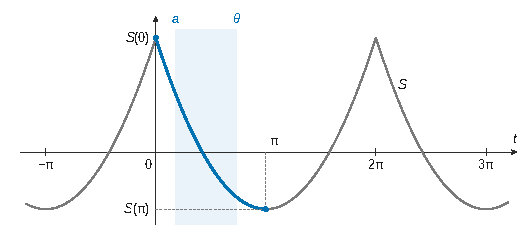
\includegraphics{figures/q5-fonction-s.pdf}
\caption*{Figure 2 --- La fonction S, paire et 2π-périodique : sur l'intervalle de
0 à π (arc bleu) elle coïncide avec t²/4 − πt/2 + S(0), obtenue sur un
segment de a à θ qui évite 0, puis par a → 0}
\end{figure}

\begin{piege}

Écrire « par convergence uniforme, on intègre terme à terme sur \([0;\theta]\) » est faux. Une limite uniforme de fonctions continues serait continue, or la somme vaut \(0\) en \(0\) et tend vers \(\frac\pi2\) en \(0^+\). Il faut s'éloigner de \(0\), puis revenir par continuité.

\end{piege}

\begin{jury}

Le rapport 2026 juge la question « fort délicate » : elle « n'a pratiquement jamais été correctement résolue ». Il propose deux voies : travailler sur des intégrales \(\int_a^b\) avec \(a,b\in\,]0;\pi[\) par convergence dominée (domination délicate), ou utiliser la question 1 en passant aux restes pour obtenir la convergence uniforme sur tout segment de \(]0;\pi[\). C'est cette seconde voie que suit la solution, la conclusion venant de la question 3 et de la continuité de \(S\) (question 4).

\end{jury}

\begin{methode}

Schéma « segment intérieur puis passage à la limite » : quand un théorème d'interversion échoue au bord d'un intervalle, on l'applique sur \([a;b]\) strictement intérieur. On fait ensuite tendre \(a\) vers le bord à l'aide d'une continuité obtenue séparément.

\end{methode}

\hypertarget{question-6}{%
\subsection{Question 6}\label{question-6}}

\begin{indication}{1}

Théorème de dérivation terme à terme pour la classe \(\mathcal C^2\) : quelles séries faut-il contrôler, et comment ?

\end{indication}

\begin{indication}{2}

Majorez \(u_n\), \(u_n'\) et \(u_n''\) uniformément en \(t\) en utilisant \(n^2+x^2\ge n^2\). Pour la relation, réduisez au même dénominateur.

\end{indication}

\hypertarget{solution-5}{%
\subsubsection{Solution}\label{solution-5}}

Fixons \(x\in\mathbb{R}\) et \(u_n(t)=\frac{\cos(nt)}{n^2(n^2+x^2)}\). Chaque \(u_n\) est de classe \(\mathcal C^2\) sur \(\mathbb{R}\), avec
\equationajustee{\begin{aligned}
u_n'(t)&=-\frac{\sin(nt)}{n(n^2+x^2)},\\
u_n''(t)&=-\frac{\cos(nt)}{n^2+x^2}.
\end{aligned}}
Pour tout \(t\in\mathbb{R}\) :
\equationajustee{\begin{aligned}
|u_n(t)|&\le\frac1{n^4},\\
|u_n'(t)|&\le\frac1{n^3},\\
|u_n''(t)|&\le\frac1{n^2}.
\end{aligned}}
Les trois séries convergent normalement, donc uniformément et en particulier simplement, sur \(\mathbb{R}\).

Le théorème de dérivation terme à terme (classe \(\mathcal C^2\)) s'applique, car ses trois hypothèses sont satisfaites :

\begin{itemize}
\tightlist
\item
  les \(u_n\) sont de classe \(\mathcal C^2\) sur \(\mathbb{R}\) ;
\item
  les séries \(\sum u_n\) et \(\sum u_n'\) convergent simplement sur \(\mathbb{R}\) ;
\item
  la série \(\sum u_n''\) converge uniformément sur \(\mathbb{R}\).
\end{itemize}

Donc \textbf{\(g_x\) est de classe \(\mathcal C^2\) sur \(\mathbb{R}\)}, et
\equationajustee{\begin{aligned}
g_x'(t)&=-\sum_{n=1}^{+\infty}\frac{\sin(nt)}{n(n^2+x^2)},\\
g_x''(t)&=-\sum_{n=1}^{+\infty}\frac{\cos(nt)}{n^2+x^2}.
\end{aligned}}
Par linéarité (séries convergentes) :
\equationajustee{\begin{aligned}
g_x''(t)-x^2g_x(t)&=-\sum_{n=1}^{+\infty}\cos(nt)\left(\frac{1}{n^2+x^2}+\frac{x^2}{n^2(n^2+x^2)}\right)\\
&=-\sum_{n=1}^{+\infty}\frac{\cos(nt)}{n^2}.
\end{aligned}}
Pour tout \(t\in\mathbb{R}\) :
\equationajustee{\boxed{g_x''(t)-x^2g_x(t)=-S(t).}}

\begin{piege}

Ne contrôler que \(\sum u_n''\) ne suffit pas : le théorème demande aussi la convergence simple de \(\sum u_n\) et de \(\sum u_n'\). Le rapport 2026 le confirme : « Quelques candidats ont oublié de mentionner la convergence simple de la série dérivée première ». Il relève aussi des confusions entre suites et séries de fonctions.

\end{piege}

\hypertarget{question-7}{%
\subsection{Question 7}\label{question-7}}

\begin{indication}{1}

Cherchez \(P(t)=at^2+bt+c\) et identifiez les coefficients. Puis vérifiez que le polynôme trouvé convient.

\end{indication}

\hypertarget{solution-6}{%
\subsubsection{Solution}\label{solution-6}}

Soit \(x\ne0\). Cherchons \(P(t)=at^2+bt+c\). Alors
\equationajustee{P''(t)-x^2P(t)=-ax^2t^2-bx^2t+(2a-cx^2).}
Il suffit que ces coefficients soient ceux de \(-\frac{t^2}{4}+\frac{\pi t}{2}-S(0)\), c'est-à-dire
\equationajustee{\begin{aligned}
-ax^2&=-\frac14,\\
-bx^2&=\frac\pi2,\\
2a-cx^2&=-S(0).
\end{aligned}}
Puisque \(x\ne0\), on prend \(a=\frac1{4x^2}\), \(b=-\frac{\pi}{2x^2}\) et \(c=\frac{2a+S(0)}{x^2}\), d'où le candidat
\equationajustee{\boxed{P(t)=\frac{t^2}{4x^2}-\frac{\pi t}{2x^2}+\frac{1}{2x^4}+\frac{S(0)}{x^2}.}}

\textbf{Vérification.} Pour tout \(t\in\mathbb{R}\),
\equationajustee{\begin{aligned}
P'(t)&=\frac{t-\pi}{2x^2},\\
P''(t)&=\frac{1}{2x^2},
\end{aligned}}
d'où
\equationajustee{\begin{aligned}
P''(t)-x^2P(t)&=\frac{1}{2x^2}-\left(\frac{t^2}{4}-\frac{\pi t}{2}+\frac{1}{2x^2}+S(0)\right)\\
&=-\frac{t^2}{4}+\frac{\pi t}{2}-S(0).
\end{aligned}}
Le polynôme \(P\), de degré \(2\), est donc bien solution de \((E_x)\) sur \(\mathbb{R}\).

\begin{jury}

On demande « une » solution : le rapport 2026 juge inutile une analyse-synthèse et précise qu'« il était donc tout à fait acceptable de parachuter un polynôme \(P\), à condition toutefois d'expliciter les calculs menant au fait qu'il est bien solution de l'équation différentielle indiquée ». D'où la vérification, avec \(P'\) et \(P''\) écrits.

\end{jury}

\begin{piege}

Le rapport 2026 juge les confusions entre conditions nécessaires et conditions suffisantes « omniprésentes » dans cette question pourtant « très simple ». L'identification fournit un candidat (condition suffisante choisie) ; c'est la vérification qui prouve qu'il convient.

\end{piege}

\hypertarget{question-8}{%
\subsection{Question 8}\label{question-8}}

\begin{indication}{1}

Les dérivées premières se lisent sur l'expression en série de \(g_x'\).

\end{indication}

\begin{indication}{2}

Sur \([0;\pi]\), la question 5 rend \(-S(t)\) polynomial, à condition d'étendre son résultat au point \(\pi\). Que dit alors la question 6 sur la restriction de \(g_x\) à \([0;\pi]\) ?

\end{indication}

\begin{indication}{3}

Écrivez \(g_x=P+Ae^{xt}+Be^{-xt}\) sur \([0;\pi]\), en justifiant cette forme. Vous ne connaissez ni \(g_x(0)\) ni \(g_x(\pi)\) ; en revanche vous connaissez deux autres valeurs.

\end{indication}

\hypertarget{solution-7}{%
\subsubsection{Solution}\label{solution-7}}

\textbf{Dérivées premières.} Soit \(x\in\mathbb{R}\). Dans l'expression de \(g_x'\) de la question 6, tous les termes sont nuls en \(0\) et en \(\pi\), car \(\sin0=\sin(n\pi)=0\) :
\equationajustee{\boxed{\begin{aligned}
g_x'(0)&=0,\\
g_x'(\pi)&=0.
\end{aligned}}}

\textbf{Résolution sur \([0;\pi]\).} Soit \(x\ne0\). Par la question 5, étendue à \(\pi\) par continuité, on a pour tout \(t\in[0;\pi]\)
\equationajustee{-S(t)=-\frac{t^2}{4}+\frac{\pi t}{2}-S(0).}
La restriction de \(g_x\) à l'intervalle \([0;\pi]\) est donc solution de \((E_x)\) sur cet intervalle.

L'équation homogène \(y''-x^2y=0\) est linéaire à coefficients constants. Son équation caractéristique \(r^2-x^2=0\) a deux racines réelles \textbf{distinctes} \(x\) et \(-x\), précisément parce que \(x\ne0\).

Les solutions de l'équation homogène sur \([0;\pi]\) sont donc les fonctions \(t\mapsto Ae^{xt}+Be^{-xt}\), avec \((A,B)\in{\mathbb{R}}^2\). En ajoutant la solution particulière \(P\), il existe \((A,B)\in{\mathbb{R}}^2\) tel que
\equationajustee{\forall t\in[0;\pi],\ g_x(t)=P(t)+Ae^{xt}+Be^{-xt}.}

\textbf{Constantes.} Pour \(t\in[0;\pi]\),
\equationajustee{g_x'(t)=\frac{t-\pi}{2x^2}+Axe^{xt}-Bxe^{-xt}.}
Les conditions \(g_x'(0)=0\) et \(g_x'(\pi)=0\) s'écrivent, après division par \(x\ne0\),
\equationajustee{\begin{aligned}
A-B&=\frac{\pi}{2x^3},\\
B&=Ae^{2\pi x}.
\end{aligned}}
Comme \(1-e^{2\pi x}\ne0\) :
\equationajustee{\begin{aligned}
A&=\frac{\pi}{2x^3(1-e^{2\pi x})},\\
B&=\frac{\pi e^{2\pi x}}{2x^3(1-e^{2\pi x})},\\
A+B&=\frac{\pi(1+e^{2\pi x})}{2x^3(1-e^{2\pi x})}.
\end{aligned}}

\textbf{Calcul de \(g_x''(0)\).} On dérive deux fois l'expression de \(g_x\) sur \([0;\pi]\) :
\equationajustee{\begin{aligned}
g_x''(0)&=P''(0)+x^2(A+B)\\
&=\frac{1}{2x^2}+\frac{\pi}{2x}\cdot\frac{1+e^{2\pi x}}{1-e^{2\pi x}}.
\end{aligned}}
En multipliant haut et bas par \(e^{-2\pi x}\) :
\equationajustee{\frac{1+e^{2\pi x}}{1-e^{2\pi x}}=-\frac{1+e^{-2\pi x}}{1-e^{-2\pi x}},}
d'où
\equationajustee{\boxed{g_x''(0)=-\frac{\pi}{2x}\times\frac{1+e^{-2\pi x}}{1-e^{-2\pi x}}+\frac{1}{2x^2}.}}

\begin{piege}

Trois erreurs classiques :

\begin{itemize}
\tightlist
\item
  résoudre \(y''-x^2y=0\) avec des sinus et cosinus (les racines caractéristiques sont réelles) ;
\item
  affirmer que \(g_x\) résout \((E_x)\) sur tout \(\mathbb{R}\) (hors de \([0;\pi]\), \(S\) n'est plus ce polynôme) ;
\item
  oublier que la question 5 n'est énoncée que sur \([0;\pi[\) alors qu'on a besoin du point \(\pi\).
\end{itemize}

\end{piege}

\begin{jury}

Le rapport 2026 regrette qu'on trouve « trop rarement » la précision que la résolution se fait sur \([0;\pi]\) et que la formule de la question 5 doit être prolongée en \(\pi\) par continuité. Il demande de justifier la forme des solutions de l'équation homogène, puisqu'il y a un paramètre \(x\) (d'où le cas \(x\ne0\)). Il ajoute : « Le choix des fonctions hyperboliques était d'ailleurs préférable à celui des exponentielles, vu les conditions aux limites. »

\end{jury}

\begin{methode}

Avec \(g_x=P+\alpha\operatorname{ch}(xt)+\beta\operatorname{sh}(xt)\), la condition \(g_x'(0)=0\) donne directement \(\beta x=-P'(0)\), et la seconde condition fixe \(\alpha\). Plus généralement, une fonction définie par une série et solution d'une équation différentielle linéaire se calcule en résolvant l'équation, puis en fixant les constantes par des valeurs lues sur la série : c'est un problème aux limites, non un problème de Cauchy.

\end{methode}

\hypertarget{question-9}{%
\subsection{Question 9}\label{question-9}}

\begin{indication}{1}

Vous disposez de deux expressions de \(g_x''(0)\) : l'une par la série de la question 6, l'autre par la question 8. Cette question se traite même si la question 8 a été admise.

\end{indication}

\begin{indication}{2}

Pour faire apparaître \(e^{2\pi x}-1\), écrivez le quotient d'exponentielles sous la forme \(1+\frac{\text{quelque chose}}{e^{2\pi x}-1}\).

\end{indication}

\hypertarget{solution-8}{%
\subsubsection{Solution}\label{solution-8}}

Soit \(x\ne0\). Par la question 6 en \(t=0\), \(g_x''(0)=-\sum_{n\ge1}\frac{1}{n^2+x^2}\). Avec la question 8, en multipliant par \(-2x^2\) :
\equationajustee{\sum_{n=1}^{+\infty}\frac{2x^2}{n^2+x^2}=\pi x\,\frac{1+e^{-2\pi x}}{1-e^{-2\pi x}}-1.}
Or, avec \(e^{2\pi x}\ne1\),
\equationajustee{\begin{aligned}
\frac{1+e^{-2\pi x}}{1-e^{-2\pi x}}&=\frac{e^{2\pi x}+1}{e^{2\pi x}-1}\\
&=1+\frac{2}{e^{2\pi x}-1}.
\end{aligned}}
D'où, pour tout \(x\in{\mathbb{R}}^*\) :
\equationajustee{\boxed{\frac{2\pi x}{e^{2\pi x}-1}=1-\pi x+\sum_{n=1}^{+\infty}\frac{2x^2}{n^2+x^2}.}}

\begin{jury}

Le rapport 2026 note que cette conclusion a souvent été réussie, mais que les calculs ont régulièrement été difficiles à suivre. Une transformation par ligne, annoncée par une phrase, suffit à rendre le calcul lisible.

\end{jury}

\begin{methode}

Le membre de gauche est \(h(2\pi x)\), avec la fonction \(h\) de la partie 2 : repérer ce lien prépare la question 12.

\end{methode}

\hypertarget{partie-2-duxe9veloppement-en-suxe9rie-entiuxe8re-de-xmapstofracxex-1-et-applications}{%
\section{\texorpdfstring{Partie 2 --- Développement en série entière de \(x\mapsto\frac{x}{e^x-1}\) et applications}{Partie 2 --- Développement en série entière de x\textbackslash mapsto\textbackslash frac\{x\}\{e\^{}x-1\} et applications}}\label{partie-2-duxe9veloppement-en-suxe9rie-entiuxe8re-de-xmapstofracxex-1-et-applications}}

On développe \(\frac{x^2}{x^2+n^2}\) en puissances de \(x^2\) avec un reste contrôlé, et l'on somme sur \(n\) : apparaissent les \(\zeta(2k)\).

Le changement de variable \(X=2\pi x\) transforme Q9 en développement de \(h\). Un produit de Cauchy fournit ensuite une récurrence sur les \(b_k\), qui donne \(\zeta(2)\) et \(\zeta(4)\).

\hypertarget{question-10}{%
\subsection{Question 10}\label{question-10}}

\begin{indication}{1}

Somme géométrique finie de raison \(-x^2/n^2\).

\end{indication}

\begin{indication}{2}

Pour la majoration, la plus grossière des minorations de \(x^2+n^2\) suffit à faire apparaître \(\zeta(2N+2)\).

\end{indication}

\hypertarget{solution-9}{%
\subsubsection{Solution}\label{solution-9}}

Soient \(x\in\,]-1;1[\), \(N\in\mathbb{N}\) et \(n\in{\mathbb{N}}^*\). Posons \(q=-\frac{x^2}{n^2}\).

On a \(q\le0\), donc \(q\ne1\), et \(1-q=\frac{n^2+x^2}{n^2}\). La somme géométrique \textbf{finie} donne
\equationajustee{\begin{aligned}
\frac1{n^2}\sum_{k=0}^{N}q^k&=\frac{1}{n^2}\cdot\frac{1-q^{N+1}}{1-q}\\
&=\frac{1}{x^2+n^2}-\frac{q^{N+1}}{x^2+n^2}.
\end{aligned}}
Et
\equationajustee{\frac{q^{N+1}}{x^2+n^2}=(-1)^{N+1}\frac{1}{x^2+n^2}\cdot\frac{x^{2N+2}}{n^{2N+2}}=R_{N,n}(x).}
D'où
\equationajustee{\boxed{\frac{1}{x^2+n^2}=\left(\frac1{n^2}\sum_{k=0}^{N}\left(\frac{-x^2}{n^2}\right)^k\right)+R_{N,n}(x).}}
Comme \(x^2+n^2\ge1\), on a \(|R_{N,n}(x)|\le\frac{|x|^{2N+2}}{n^{2N+2}}\).

La série de Riemann \(\sum n^{-(2N+2)}\) converge, de somme \(\zeta(2N+2)\). Par comparaison de séries à termes positifs, \(\sum_n|R_{N,n}(x)|\) converge et
\equationajustee{\boxed{\sum_{n=1}^{+\infty}|R_{N,n}(x)|\le\zeta(2N+2)\,|x|^{2N+2}.}}

\begin{jury}

Le rapport 2026 regrette que beaucoup passent par des sommes géométriques infinies, inutiles ici, et que « peu de candidats ont pensé à justifier la convergence de la série indiquée, se limitant à un calcul formel ». Avant d'écrire la somme d'une série dans une inégalité, on établit sa convergence : ici par comparaison de séries à termes positifs.

\end{jury}

\hypertarget{question-11}{%
\subsection{Question 11}\label{question-11}}

\begin{indication}{1}

Pour \(\zeta(s)\to1\), isolez le terme \(n=1\) et majorez \(\sum_{n\ge2}n^{-s}\) par une quantité qui tend vers \(0\), en factorisant \(n^{-2}\).

\end{indication}

\begin{indication}{2}

Multipliez l'identité de Q10 par \(x^2\) et sommez sur \(n\) à \(N\) fixé : quelle propriété permet d'échanger \(\sum_n\) et une somme finie sur \(k\) ?

Puis faites tendre \(N\) vers \(+\infty\).

\end{indication}

\hypertarget{solution-10}{%
\subsubsection{Solution}\label{solution-10}}

\textbf{Limite de \(\zeta\).} Pour \(s\ge2\) et \(n\ge2\),
\equationajustee{\frac1{n^s}\le\frac1{2^{s-2}}\cdot\frac{1}{n^2}.}
En sommant ces inégalités entre termes de séries convergentes,
\equationajustee{\begin{aligned}
0\le\zeta(s)-1&=\sum_{n=2}^{+\infty}\frac{1}{n^s}\\
&\le\frac{\zeta(2)-1}{2^{s-2}}.
\end{aligned}}
Ce majorant tend vers \(0\), donc \(\lim_{s\to+\infty}\zeta(s)=1\). En particulier, \((\zeta(2N+2))_N\) est bornée.

\textbf{Sommation.} Soit \(x\in\,]-1;1[\). En multipliant Q10 par \(x^2\) et en posant \(j=k+1\) :
\equationajustee{\frac{x^2}{x^2+n^2}=\sum_{j=1}^{N+1}(-1)^{j+1}\frac{x^{2j}}{n^{2j}}+x^2R_{N,n}(x).}
Les séries \(\sum_nn^{-2j}\) et \(\sum_nR_{N,n}(x)\) convergent ; la somme sur \(j\) étant finie, la linéarité donne
\equationajustee{\begin{aligned}
\sum_{n=1}^{+\infty}\frac{x^2}{x^2+n^2}&=\sum_{j=1}^{N+1}(-1)^{j+1}\zeta(2j)x^{2j}\\
&\quad+x^2\sum_{n=1}^{+\infty}R_{N,n}(x).
\end{aligned}}
Le dernier terme est majoré en module par \(x^2\zeta(2N+2)|x|^{2N+2}\), qui tend vers \(0\) car \(|x|<1\). Les sommes partielles de \(\sum(-1)^{k+1}\zeta(2k)x^{2k}\) convergent donc. Pour tout \(x\in\,]-1;1[\) :
\equationajustee{\boxed{\begin{aligned}{}&\sum_{n=1}^{+\infty}\frac{x^2}{x^2+n^2}\\
&\quad=\sum_{k=1}^{+\infty}(-1)^{k+1}\zeta(2k)x^{2k}.
\end{aligned}}}

\begin{piege}

Pour la limite de \(\zeta\), la convergence normale de \(\sum n^{-s}\) a lieu sur \([2;+\infty[\), jamais près de \(1\). Le rapport 2026 le souligne : une convergence uniforme près de \(1\) donnerait, par double limite, la convergence de la série harmonique.

Si l'on invoque le théorème de la double limite en \(+\infty\), il faut justifier la convergence terme à terme \emph{avant} de conclure ; la continuité des termes est, elle, hors sujet pour une limite en \(+\infty\). La majoration élémentaire ci-dessus évite ces écueils.

\end{piege}

\begin{jury}

Pour la seconde partie, le rapport 2026 attend une sommation de l'identité de Q10 avec une justification soigneuse des convergences, puis la majoration de Q10 pour conclure : « Trop de candidats se sont pourtant permis des interversions de sommes infinies sans justification. »

\end{jury}

\begin{methode}

Pour intervertir deux sommations sans théorème de sommation double, on tronque l'une d'elles (somme finie, linéarité), on contrôle le reste uniformément, puis on passe à la limite. C'est exactement le rôle du reste \(R_{N,n}\).

\end{methode}

\hypertarget{question-12}{%
\subsection{Question 12}\label{question-12}}

\begin{indication}{1}

Dans la question 9, le membre de gauche est \(h\) évalué en un point bien choisi. Posez \(X=2\pi x\) : à quelle condition sur \(X\) peut-on appliquer la question 11 ?

\end{indication}

\begin{indication}{2}

Le point \(X=0\) est exclu de la question 9 : traitez-le à part. Pour les \(b_k\), reliez les coefficients d'une série entière aux dérivées de sa somme en \(0\).

\end{indication}

\hypertarget{solution-11}{%
\subsubsection{Solution}\label{solution-11}}

Soit \(X\in\,]-2\pi;2\pi[\) avec \(X\ne0\). Posons \(x=\frac{X}{2\pi}\), de sorte que \(x\in\,]-1;1[\setminus\{0\}\).

La lettre \(X\) est réservée à la variable de \(h\), la lettre \(x\) à celle des questions 9 et 11. La question 9 s'écrit
\equationajustee{h(X)=1-\frac X2+2\sum_{n=1}^{+\infty}\frac{x^2}{n^2+x^2},}
et la question 11 donne
\equationajustee{\begin{aligned}
h(X)&=1-\frac X2+2\sum_{k=1}^{+\infty}(-1)^{k+1}\zeta(2k)\frac{X^{2k}}{(2\pi)^{2k}}\\
&=1-\frac X2+\sum_{k=1}^{+\infty}(-1)^{k+1}\frac{\zeta(2k)}{2^{2k-1}\pi^{2k}}X^{2k}.
\end{aligned}}
En \(X=0\), les deux membres valent \(1\). Donc, pour tout \(x\in\,]-2\pi;2\pi[\) :
\equationajustee{\boxed{h(x)=1-\frac12x+\sum_{k=1}^{+\infty}(-1)^{k+1}\frac{\zeta(2k)}{2^{2k-1}\pi^{2k}}x^{2k}.}}
La série entière converge en tout point de \(]-2\pi;2\pi[\), donc son rayon est au moins \(2\pi\) : \textbf{\(h\) est développable en série entière}.

La somme d'une série entière \(\sum a_mx^m\) est \(\mathcal C^\infty\) sur l'intervalle ouvert de convergence et \(a_m=\frac{h^{(m)}(0)}{m!}\). Donc \(b_m=m!\,a_m\) :
\equationajustee{\boxed{\begin{aligned}
b_0&=1,\\
b_1&=-\frac12,\\
b_{2k}&=(-1)^{k+1}\frac{(2k)!\,\zeta(2k)}{2^{2k-1}\pi^{2k}}\ \ (k\ge1),\\
b_{2k+1}&=0\ \ (k\ge1).
\end{aligned}}}

\begin{piege}

Ne pas confondre le coefficient \(a_m\) et la dérivée \(b_m=h^{(m)}(0)=m!\,a_m\) : l'oubli du facteur \((2k)!\) fausse \(\zeta(2)\) en question 14.

Et \(b_1=-\frac12\ne0\) : la nullité ne concerne que les \(b_{2k+1}\) avec \(k\ge1\).

\end{piege}

\begin{jury}

Le rapport 2026 reproche des rédactions confuses : très peu de candidats ont introduit et nommé leurs variables (utiliser à la fois \(x\) pour le développement de la question 11 et \(h(x)\) n'est « pas une bonne idée »), et peu ont examiné le cas \(x=0\). Les expressions des \(b_i\), une fois la formule admise, ont en revanche souvent été trouvées.

\end{jury}

\hypertarget{question-13}{%
\subsection{Question 13}\label{question-13}}

\begin{indication}{1}

Suivez l'indication : \(h(x)\cdot\frac{e^x-1}{x}=1\). Développez \(\frac{e^x-1}{x}\) en série entière.

\end{indication}

\begin{indication}{2}

Produit de Cauchy de deux séries entières, en précisant les rayons, puis unicité des coefficients d'un développement en série entière.

\end{indication}

\hypertarget{solution-12}{%
\subsubsection{Solution}\label{solution-12}}

Sur \(]-2\pi;2\pi[\), \(h(x)=\sum_{k\ge0}\frac{b_k}{k!}x^k\), série entière de rayon \(R_1\ge2\pi\) (question 12).

Pour tout réel \(x\), posons \(\varphi(x)=\sum_{j\ge0}\frac{x^j}{(j+1)!}\). Cette série entière a un rayon infini, et la série de l'exponentielle donne \(\varphi(x)=\frac{e^x-1}{x}\) si \(x\ne0\), \(\varphi(0)=1\).

Rappelons le théorème sur le produit de Cauchy. Soient \(\sum\alpha_kx^k\) et \(\sum\beta_jx^j\) deux séries entières de rayons \(R_1\) et \(R_2\), et \(c_n=\sum_{k=0}^{n}\alpha_k\beta_{n-k}\).

Alors la série entière \(\sum c_nx^n\) a un rayon au moins \(\min(R_1,R_2)\), et pour \(|x|<\min(R_1,R_2)\) sa somme est le produit des deux sommes.

Ici \(\min(R_1,+\infty)\ge2\pi\), donc pour tout \(x\in\,]-2\pi;2\pi[\) :
\equationajustee{h(x)\varphi(x)=\sum_{n=0}^{+\infty}c_nx^n,}
avec
\equationajustee{c_n=\sum_{k=0}^{n}\frac{b_k}{k!\,(n+1-k)!}.}
Or \(h(x)\varphi(x)=1\) pour tout \(x\in\,]-2\pi;2\pi[\), \(x=0\) compris.

Par unicité des coefficients, \(c_0=1\) et \(c_n=0\) pour \(n\ge1\). Pour tout \(n\in{\mathbb{N}}^*\) :
\equationajustee{\boxed{\sum_{k=0}^{n}\frac{b_k}{k!\,(n+1-k)!}=0.}}

\begin{jury}

D'après le rapport 2026, l'indication a très rarement été exploitée, et presque jamais avec une justification précise : les rayons de convergence n'étaient en général pas cités (il n'était pas nécessaire de les calculer exactement), ni « l'énoncé précis du théorème sur les produits de Cauchy de séries entières ». La question n'était pourtant pas profondément difficile.

\end{jury}

\begin{piege}

Le second facteur est \(\sum\frac{x^j}{(j+1)!}\), pas \(\sum\frac{x^j}{j!}\) : un décalage d'indice ici rend toute la question 14 incohérente.

\end{piege}

\hypertarget{question-14}{%
\subsection{Question 14}\label{question-14}}

\begin{indication}{1}

Écrivez la relation de la question 13 pour \(n=2\), puis pour \(n=4\) (en utilisant \(b_3=0\)).

\end{indication}

\begin{indication}{2}

Ensuite, identifiez avec l'expression de \(b_{2k}\) de la question 12 pour \(k=1\) et \(k=2\).

\end{indication}

\hypertarget{solution-13}{%
\subsubsection{Solution}\label{solution-13}}

Pour \(n=1\) (contrôle) : \(\frac{b_0}{2!}+\frac{b_1}{1!\,1!}=\frac12-\frac12=0\).

Pour \(n=2\) :
\equationajustee{\begin{aligned}
\frac{b_0}{3!}+\frac{b_1}{1!\,2!}+\frac{b_2}{2!\,1!}&=\frac16-\frac14+\frac{b_2}{2}\\
&=0,
\end{aligned}}
donc \(\boxed{b_2=\frac16}\).

Pour \(n=4\), avec \(b_3=0\) :
\equationajustee{\begin{aligned}
0&=\frac{b_0}{5!}+\frac{b_1}{1!\,4!}+\frac{b_2}{2!\,3!}+\frac{b_4}{4!\,1!}\\
&=\frac{1}{120}-\frac{1}{48}+\frac{1}{72}+\frac{b_4}{24}\\
&=\frac{6-15+10}{720}+\frac{b_4}{24},
\end{aligned}}
donc \(b_4=-\frac{24}{720}\), soit \(\boxed{b_4=-\frac1{30}}\).

Par la question 12, avec \(k=1\) puis \(k=2\) :
\equationajustee{\begin{aligned}
b_2&=\frac{2!\,\zeta(2)}{2\pi^2}=\frac{\zeta(2)}{\pi^2},\\
b_4&=-\frac{4!\,\zeta(4)}{8\pi^4}=-\frac{3\zeta(4)}{\pi^4}.
\end{aligned}}
D'où
\equationajustee{\boxed{\begin{aligned}
\zeta(2)&=\frac{\pi^2}{6},\\
\zeta(4)&=\frac{\pi^4}{90}.
\end{aligned}}}

\begin{piege}

Contrôlez le signe : \(\zeta(4)>1\). Le rapport 2026 rapporte que « Certains ont trouvé sans sourciller une valeur négative pour \(\zeta(4)\) ! ». Ici \(b_4<0\) et le facteur \((-1)^{k+1}\) vaut \(-1\) pour \(k=2\) : les deux signes se compensent.

\end{piege}

\begin{jury}

Le rapport 2026 indique que \(b_2\) et \(\zeta(2)\) ont été souvent obtenus, mais rarement \(b_4\) et \(\zeta(4)\). Puisque \(b_3=0\), « il fallait en tirer profit et appliquer directement la formule de la question 13 au rang 4, à partir de la connaissance de \(b_2\) ».

\end{jury}

\begin{methode}

Sans calculatrice, posez un dénominateur commun (\(720\)) et vérifiez la relation sur le cas \(n=1\) avant de l'utiliser : c'est un test gratuit de la formule de Q13 et des valeurs de \(b_0\), \(b_1\).

\end{methode}

\hypertarget{partie-3-probabilituxe9-quun-entier-naturel-choisi-au-hasard-et-uniformuxe9ment-dans-1n-soit-sans-facteur-uxe0-la-puissance-k}{%
\section{\texorpdfstring{Partie 3 --- Probabilité qu'un entier naturel choisi au hasard et uniformément dans \([\![1;n]\!]\) soit sans facteur à la puissance \(k\)}{Partie 3 --- Probabilité qu'un entier naturel choisi au hasard et uniformément dans {[}\textbackslash!{[}1;n{]}\textbackslash!{]} soit sans facteur à la puissance k}}\label{partie-3-probabilituxe9-quun-entier-naturel-choisi-au-hasard-et-uniformuxe9ment-dans-1n-soit-sans-facteur-uxe0-la-puissance-k}}

On démontre la formule du crible par les indicatrices (Q15--Q17), on l'applique aux événements « \(p_i^k\) divise l'entier tiré » (Q18), on réécrit le résultat avec la fonction de Möbius (Q19), puis on passe à la limite \(n\to+\infty\) par convergence dominée (Q20).

\hypertarget{question-15}{%
\subsection{Question 15}\label{question-15}}

\begin{indication}{1}

Développer le produit revient à choisir, dans chaque facteur, soit \(1\), soit \(x_i\). Quels termes obtient-on ?

\end{indication}

\begin{indication}{2}

Pour une preuve par récurrence sur \(r\), notez \(\Sigma_m^{(r)}\) la somme des produits de \(m\) facteurs d'indices strictement croissants.

Reliez ensuite \(\Sigma_m^{(r+1)}\) à \(\Sigma_m^{(r)}\) et \(\Sigma_{m-1}^{(r)}\) en distinguant si l'indice \(r+1\) est utilisé.

\end{indication}

\hypertarget{solution-14}{%
\subsubsection{Solution}\label{solution-14}}

Soit \((x_1,\dots,x_r)\in{\mathbb{R}}^r\). Pour \(1\le m\le r\), notons
\equationajustee{\Sigma_m^{(r)}=\sum_{i_1<\dots<i_m}x_{i_1}\cdots x_{i_m}\qquad(\text{indices dans }[\![1;r]\!]),}
avec \(\Sigma_0^{(r)}=1\) et \(\Sigma_m^{(r)}=0\) si \(m>r\). Montrons par récurrence que \(\prod_{i=1}^{r}(1+x_i)=\sum_{m=0}^{r}\Sigma_m^{(r)}\).

Pour \(r=1\) : \(1+x_1=\Sigma_0^{(1)}+\Sigma_1^{(1)}\).

Hérédité. En séparant les \(m\)-uplets selon que \(i_m=r+1\) ou \(i_m\le r\), on obtient pour \(1\le m\le r+1\)
\equationajustee{\Sigma_m^{(r+1)}=\Sigma_m^{(r)}+x_{r+1}\Sigma_{m-1}^{(r)}.}
Avec \(\Sigma_{r+1}^{(r)}=0\) et l'hypothèse de récurrence :
\equationajustee{\begin{aligned}
\sum_{m=0}^{r+1}\Sigma_m^{(r+1)}&=\sum_{m=0}^{r}\Sigma_m^{(r)}+x_{r+1}\sum_{m=0}^{r}\Sigma_m^{(r)}\\
&=(1+x_{r+1})\prod_{i=1}^{r}(1+x_i).
\end{aligned}}
Ainsi, pour tout \(r\in{\mathbb{N}}^*\) et tout \((x_1,\dots,x_r)\in{\mathbb{R}}^r\) :
\equationajustee{\boxed{\begin{aligned}{}&\prod_{i=1}^{r}(1+x_i)\\
&\quad=1+\sum_{m=1}^{r}\left(\sum_{1\le i_1<\dots<i_m\le r}x_{i_1}x_{i_2}\cdots x_{i_m}\right).
\end{aligned}}}

\begin{jury}

Le rapport 2026 trouve les rédactions soit « excessivement pointilleuses » (récurrences très lourdes), soit trop vagues. Il précise : « On acceptait tout à fait un raisonnement consistant à s'interroger sur la forme générale des termes issus du produit ». En développant, chaque terme correspond au choix des facteurs où l'on prend \(x_i\) (indices \(i_1<\dots<i_m\)) et de ceux où l'on prend \(1\) ; chaque partie de \([\![1;r]\!]\) apparaît une fois. La récurrence ci-dessus reste une rédaction sûre, à condition de rester légère.

\end{jury}

\hypertarget{question-16}{%
\subsection{Question 16}\label{question-16}}

\begin{indication}{1}

Ce sont des égalités de fonctions sur \(\Omega\) : évaluez en une issue \(\omega\) quelconque et distinguez des cas.

\end{indication}

\hypertarget{solution-15}{%
\subsubsection{Solution}\label{solution-15}}

Les deux égalités sont des égalités de fonctions sur \(\Omega\) ; soit \(\omega\in\Omega\) une issue.

Si \(\omega\in A\) : \(\mathbf 1_{\bar A}(\omega)=0=1-\mathbf 1_A(\omega)\). Sinon : \(\mathbf 1_{\bar A}(\omega)=1=1-\mathbf 1_A(\omega)\). Donc \(\boxed{\mathbf 1_{\bar A}=1-\mathbf 1_A}\).

Les nombres \(\mathbf 1_{A_i}(\omega)\) valent \(0\) ou \(1\).

Leur produit vaut \(1\) si et seulement si tous valent \(1\), c'est-à-dire si \(\omega\in A_1\cap\dots\cap A_m\) ; il vaut \(0\) sinon.

Donc \(\boxed{\mathbf 1_{A_1}\mathbf 1_{A_2}\cdots\mathbf 1_{A_m}=\mathbf 1_{A_1\cap A_2\cap\dots\cap A_m}}\).

\begin{piege}

Une issue \(\omega\) est un élément de \(\Omega\) ; un événement est un ensemble d'issues. Le rapport 2026 juge que de telles confusions « ruinent toute possibilité de raisonnement ». Il note aussi qu'« Un nombre très important de candidats s'est mis à parler d'indépendance d'événements, ce qui était tout à fait hors-sujet. »

\end{piege}

\hypertarget{question-17}{%
\subsection{Question 17}\label{question-17}}

\begin{indication}{1}

Passez au complémentaire de la réunion et utilisez De Morgan pour obtenir un produit d'indicatrices.

\end{indication}

\begin{indication}{2}

Appliquez la question 15 avec un choix de \(x_i\) faisant apparaître les signes, puis prenez l'espérance.

\end{indication}

\hypertarget{solution-16}{%
\subsubsection{Solution}\label{solution-16}}

Par De Morgan et la question 16,
\equationajustee{\begin{aligned}
\mathbf 1_{A_1\cup\dots\cup A_r}&=1-\mathbf 1_{\bar A_1\cap\dots\cap\bar A_r}\\
&=1-\prod_{i=1}^{r}(1-\mathbf 1_{A_i}).
\end{aligned}}
On applique la question 15 en chaque \(\omega\) avec \(x_i=-\mathbf 1_{A_i}(\omega)\), puis la question 16 :
\equationajustee{\begin{aligned}{}&\prod_{i=1}^{r}(1-\mathbf 1_{A_i})\\
&\quad=1+\sum_{m=1}^{r}(-1)^m\sum_{1\le i_1<\dots<i_m\le r}\mathbf 1_{A_{i_1}\cap\dots\cap A_{i_m}}.
\end{aligned}}
Donc
\equationajustee{\begin{aligned}{}&\mathbf 1_{A_1\cup\dots\cup A_r}\\
&\quad=\sum_{m=1}^{r}(-1)^{m+1}\sum_{1\le i_1<\dots<i_m\le r}\mathbf 1_{A_{i_1}\cap\dots\cap A_{i_m}}.
\end{aligned}}
Ces variables aléatoires sont bornées, donc d'espérance finie. Par linéarité de l'espérance (somme finie) et \(E(\mathbf 1_B)=P(B)\) :
\equationajustee{\boxed{\begin{aligned}{}&P(A_1\cup\dots\cup A_r)\\
&\quad=\sum_{m=1}^{r}(-1)^{m+1}\left(\sum_{1\le i_1<\dots<i_m\le r}P(A_{i_1}\cap\dots\cap A_{i_m})\right).
\end{aligned}}}

\begin{jury}

Le rapport 2026 est explicite : « La formulation de la question exigeait une utilisation des indicatrices », et non une récurrence fondée sur la formule du crible à deux termes. Il relève de nombreuses confusions entre les événements et leurs espérances : on prend l'espérance d'une \textbf{variable aléatoire} (l'indicatrice), jamais d'un événement.

\end{jury}

\begin{piege}

Citer la formule du crible comme résultat de cours ne répond pas : l'énoncé demande de la déduire de Q15 et Q16. Le signe \(-\) dans \(x_i=-\mathbf 1_{A_i}\) est ce qui produit les \((-1)^m\).

\end{piege}

\hypertarget{question-18}{%
\subsection{Question 18}\label{question-18}}

\begin{indication}{1}

Décrivez le complémentaire de \(S_n(k)\) dans \([\![1;n]\!]\) à l'aide des \(A_n(p_i^k)\).

\end{indication}

\begin{indication}{2}

Après la question 17, il reste à identifier une intersection \(A_n(a)\cap A_n(b)\cap\dots\) comme un seul \(A_n(\cdot)\) : que dire de puissances \(k\)-ièmes de nombres premiers distincts ?

\end{indication}

\hypertarget{solution-17}{%
\subsubsection{Solution}\label{solution-17}}

Un \(m\in[\![1;n]\!]\) n'est pas dans \(S_n(k)\) si et seulement si \(p_j^k\mid m\) pour un \(j\in[\![1;r]\!]\), c'est-à-dire \(m\in\bigcup_iA_n(p_i^k)\). Donc
\equationajustee{\boxed{q_n(k)=1-P_n\left(\bigcup_{i=1}^{r}A_n(p_i^k)\right).}}
Se limiter à \(p_1,\dots,p_r\) ne perd rien : si \(p\) premier vérifie \(p^k\mid m\le n\), alors \(p\le m\le n\).

La question 17 donne
\equationajustee{\begin{aligned}
q_n(k)&=1-\sum_{m=1}^{r}(-1)^{m+1}\sum_{1\le i_1<\dots<i_m\le r}P_n\left(\bigcap_{\ell=1}^{m}A_n(p_{i_\ell}^k)\right)\\
&=1+\sum_{m=1}^{r}\sum_{1\le i_1<\dots<i_m\le r}(-1)^mP_n\left(\bigcap_{\ell=1}^{m}A_n(p_{i_\ell}^k)\right).
\end{aligned}}
Soit \(j\in[\![1;n]\!]\) tel que chaque \(p_{i_\ell}^k\) divise \(j\). Les \(p_{i_\ell}\) sont des nombres premiers \textbf{deux à deux distincts} : la décomposition en facteurs premiers de \(j\) contient chacun d'eux avec un exposant au moins \(k\).

Donc \(p_{i_1}^k\cdots p_{i_m}^k\mid j\) ; la réciproque est immédiate. Ainsi \(\bigcap_\ell A_n(p_{i_\ell}^k)=A_n(p_{i_1}^k\cdots p_{i_m}^k)\) et
\equationajustee{\boxed{\begin{aligned}{}&q_n(k)\\
&\quad=1+\sum_{m=1}^{r}\sum_{1\le i_1<i_2<\dots<i_m\le r}(-1)^m\,P_n\left(A_n\left(p_{i_1}^kp_{i_2}^k\cdots p_{i_m}^k\right)\right).
\end{aligned}}}

\begin{jury}

Selon le rapport 2026, la clé était l'égalité \(A(p_{i_1}^k\cdots p_{i_m}^k)=A(p_{i_1}^k)\cap\cdots\cap A(p_{i_m}^k)\), qui relève de l'arithmétique élémentaire à condition d'insister sur le fait que les \(p_{i_\ell}\) sont des nombres premiers \emph{deux à deux distincts}. Peu de candidats sont allés au-delà du début de la question.

\end{jury}

\begin{piege}

Le passage \(-(-1)^{m+1}=(-1)^m\) est une source classique d'erreur de signe. Et « divisible par \(a\) et par \(b\) » n'entraîne pas en général « divisible par \(ab\) » (pour \(a=b=2\), l'entier \(2\) convient) : ici, c'est la décomposition en facteurs premiers, avec des nombres premiers deux à deux distincts, qui le justifie.

\end{piege}

\hypertarget{question-19}{%
\subsection{Question 19}\label{question-19}}

\begin{indication}{1}

Combien \([\![1;n]\!]\) contient-il de multiples de \(d\) ?

\end{indication}

\begin{indication}{2}

Posez \(D=p_{i_1}\cdots p_{i_m}\) : que vaut \(\mu(D)\) ? Puis expliquez pourquoi tous les autres entiers \(d\) apportent une contribution nulle à la somme infinie.

\end{indication}

\hypertarget{solution-18}{%
\subsubsection{Solution}\label{solution-18}}

Les multiples de \(d\) dans \([\![1;n]\!]\) sont \(d,2d,\dots,\lfloor n/d\rfloor d\), donc \(P_n(A_n(d))=\frac1n\left\lfloor\frac nd\right\rfloor\).

Pour \(i_1<\dots<i_m\), l'entier \(D=p_{i_1}\cdots p_{i_m}\) vérifie \(p_{i_1}^k\cdots p_{i_m}^k=D^k\) et \(\mu(D)=(-1)^m\).

L'application \(\{i_1<\dots<i_m\}\mapsto D\) est injective (unicité de la décomposition). Son image est l'ensemble \(\mathcal D\) des entiers \(D>1\) sans facteur carré dont les facteurs premiers sont parmi \(p_1,\dots,p_r\).

Le terme \(1\) vaut \(\frac1n\mu(1)\lfloor n/1^k\rfloor\). D'où
\equationajustee{q_n(k)=\frac1n\sum_{D\in\{1\}\cup\mathcal D}\mu(D)\left\lfloor\frac{n}{D^k}\right\rfloor.}
Soit \(d\notin\{1\}\cup\mathcal D\).

\begin{itemize}
\tightlist
\item
  Ou bien \(d\) a un facteur carré, et \(\mu(d)=0\).
\item
  Ou bien \(d\) a un facteur premier \(p>n\). Alors \(d^k\ge d\ge p>n\), donc \(\lfloor n/d^k\rfloor=0\).
\end{itemize}

Ces termes sont nuls, la somme n'a qu'un nombre fini de termes non nuls, et
\equationajustee{\boxed{q_n(k)=\frac1n\sum_{d=1}^{+\infty}\mu(d)\left\lfloor\frac{n}{d^k}\right\rfloor.}}

\begin{jury}

Le rapport 2026 : « Cette difficile question n'a pratiquement jamais été correctement résolue » ; il fallait organiser avec une grande minutie les termes du résultat de la question 18. Ici, cette organisation tient en trois points : le changement d'indice \(D=p_{i_1}\cdots p_{i_m}\), son injectivité, et la nullité de tous les autres termes.

\end{jury}

\begin{methode}

Pour étendre une somme finie à une somme sur tout \({\mathbb{N}}^*\), on montre que chaque terme ajouté est nul ; la « série » obtenue est alors à support fini et sa convergence est sans objet.

\end{methode}

\hypertarget{question-20}{%
\subsection{Question 20}\label{question-20}}

\begin{indication}{1}

Exprimez \(q_n(k)\) comme une intégrale de \(f_n\) sur \([1;+\infty[\), et cherchez la limite simple de \(f_n(t)\) à \(t\) fixé, en encadrant la partie entière.

\end{indication}

\begin{indication}{2}

Pour la domination, majorez \(|f_n(t)|\) par une fonction de \(t\) seule, et justifiez son intégrabilité en revenant à une série.

\end{indication}

\hypertarget{solution-19}{%
\subsubsection{Solution}\label{solution-19}}

La série \(\ell=\sum_{d\ge1}\frac{\mu(d)}{d^k}\) converge absolument, car \(|\mu(d)|d^{-k}\le d^{-k}\) et \(k\ge2\).

\textbf{Intégrales.} \(f_n\) est constante sur chaque \([d;d+1[\), donc continue par morceaux. Elle est nulle sur \([n+1;+\infty[\), car \(\lfloor n/d^k\rfloor=0\) pour \(d>n\). Elle est donc intégrable et, par Q19,
\equationajustee{\begin{aligned}
\int_1^{+\infty}f_n(t)\,\mathrm{d}t&=\sum_{d=1}^{n}\frac1n\mu(d)\left\lfloor\frac{n}{d^k}\right\rfloor\\
&=q_n(k).
\end{aligned}}

\textbf{Convergence simple.} Soit \(t\ge1\) et \(d=\lfloor t\rfloor\). De l'encadrement \(\frac{n}{d^k}-1<\left\lfloor\frac{n}{d^k}\right\rfloor\le\frac{n}{d^k}\) on tire
\equationajustee{\frac{1}{d^k}-\frac1n<\frac1n\left\lfloor\frac{n}{d^k}\right\rfloor\le\frac1{d^k}.}
Donc \(f_n(t)\to f(t)=\frac{\mu(\lfloor t\rfloor)}{\lfloor t\rfloor^k}\), fonction continue par morceaux.

\textbf{Domination.} On a \(|f_n(t)|\le\frac{1}{\lfloor t\rfloor^k}\), et l'on pose \(\varphi(t)=\frac{1}{\lfloor t\rfloor^k}\) : fonction indépendante de \(n\), positive, continue par morceaux.

Elle est intégrable sur \([1;+\infty[\) : pour \(X\ge1\),
\equationajustee{\begin{aligned}
\int_1^X\varphi&\le\int_1^{\lfloor X\rfloor+1}\varphi\\
&=\sum_{d=1}^{\lfloor X\rfloor}\frac{1}{d^k}\\
&\le\zeta(k),
\end{aligned}}
et ces intégrales sont croissantes en \(X\) et majorées. (Variante : \(t<d+1\le2d\) donne \(\varphi(t)\le\frac{2^k}{t^k}\), intégrale de Riemann convergente.)

\begin{figure}[H]
\centering
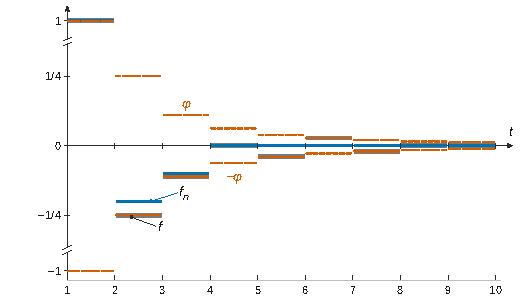
\includegraphics{figures/q20-escalier-domination.pdf}
\caption*{Figure 3 --- Pour k = 2 et n = 10, la fonction en escalier f\_n (bleu),
sa limite simple f (gris) et la domination −φ ≤ f\_n ≤ φ avec φ(t) =
1/⌊t⌋\^{}k (tirets)}
\end{figure}

\textbf{Conclusion.} Par le théorème de convergence dominée,
\equationajustee{q_n(k)=\int_1^{+\infty}f_n\xrightarrow[n\to+\infty]{}\int_1^{+\infty}f.}
Et, \(f\) étant intégrable,
\equationajustee{\begin{aligned}
\int_1^{+\infty}f&=\lim_{M\to+\infty}\int_1^{M+1}f\\
&=\lim_{M\to+\infty}\sum_{d=1}^{M}\frac{\mu(d)}{d^k}\\
&=\ell.
\end{aligned}}
Donc \textbf{la suite \((q_n(k))_{n\in{\mathbb{N}}^*}\) converge} et
\equationajustee{\boxed{\lim_{n\to+\infty}q_n(k)=\sum_{d=1}^{+\infty}\frac{\mu(d)}{d^k}.}}

\begin{piege}

La majoration \(|f_n(t)|\le\frac1{\lfloor t\rfloor^k}\) est une domination parfaitement valable : une fonction en escalier positive est intégrable dès que la série de ses marches converge. L'erreur à éviter est d'écrire « \(|f_n(t)|\le\frac1{d^k}\) » sans dire que \(d=\lfloor t\rfloor\) dépend de \(t\), et sans prouver l'intégrabilité de la fonction obtenue.

\end{piege}

\begin{jury}

Le rapport 2026 explique le rôle de l'indication : elle contourne l'absence au programme d'un théorème de double limite pour une variable entière. Mais « Le lien entre convergence dominée et la situation présente n'a essentiellement pas été vu » par les rares candidats arrivés jusque-là.

\end{jury}

\begin{methode}

Transformer une somme en intégrale d'une fonction en escalier permet d'utiliser le théorème de convergence dominée pour intervertir limite et somme infinie : c'est l'usage que suggère l'indication.

\end{methode}

\hypertarget{partie-4-calcul-de-la-somme-sum_d1inftyfracmuddk}{%
\section{\texorpdfstring{Partie 4 --- Calcul de la somme \(\sum_{d=1}^{+\infty}\frac{\mu(d)}{d^k}\)}{Partie 4 --- Calcul de la somme \textbackslash sum\_\{d=1\}\^{}\{+\textbackslash infty\}\textbackslash frac\{\textbackslash mu(d)\}\{d\^{}k\}}}\label{partie-4-calcul-de-la-somme-sum_d1inftyfracmuddk}}

On veut le produit de deux séries \(\left(\sum u_i\right)\left(\sum v_j\right)\) regroupé selon le produit \(ij=m\). Sans théorème sur les familles sommables, on compare des sommes finies indexées par le carré \(E_N\) et par la région \(F_N\) sous l'hyperbole \(ij=N\). La propriété \(\sum_{d\mid m}\mu(d)=[m=1]\) conclut.

\hypertarget{question-21}{%
\subsection{Question 21}\label{question-21}}

\begin{indication}{1}

Pour les inclusions, majorez \(ij\) quand \((i,j)\in E_N\). Puis réécrivez \(S_N\) comme une somme indexée par \(F_N\) grâce à un changement d'indices \((m,d)\mapsto(\dots)\).

\end{indication}

\begin{indication}{2}

\((S_N)\) est croissante : majorez-la. Pour l'identité, encadrez le produit des sommes partielles entre \(S_N\) et \(S_{N^2}\).

\end{indication}

\hypertarget{solution-20}{%
\subsubsection{Solution}\label{solution-20}}

\textbf{Inclusions.} \(F_N\subset E_N\) par définition. Si \((i,j)\in E_N\), alors \(1\le i,j\le N\le N^2\) et \(ij\le N^2\), donc \((i,j)\in F_{N^2}\) :
\equationajustee{\boxed{F_N\subset E_N\subset F_{N^2}.}}

\begin{figure}[H]
\centering
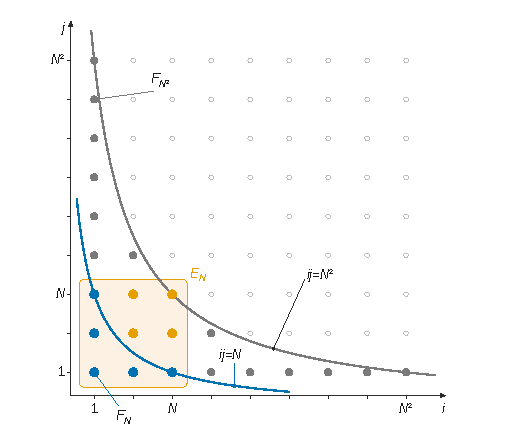
\includegraphics{figures/q21-domaines-fn-en.pdf}
\caption*{Figure 4 --- Pour N = 3, F\_N (bleu) sous l'hyperbole ij = N, le carré
E\_N (orange pour E\_N privé de F\_N) et F\_N² (gris) sous l'hyperbole
ij = N², qui passe par le coin (N, N)}
\end{figure}

\textbf{Réindexation.} \((m,d)\mapsto(d,m/d)\) est une bijection de \(\{(m,d):1\le m\le N,\ d\mid m\}\) sur \(F_N\), de réciproque \((i,j)\mapsto(ij,i)\). Donc \(S_N=\sum_{(i,j)\in F_N}|u_i|v_j\).

\textbf{Convergence.} Les termes sont positifs et \(F_N\subset F_{N+1}\) : \((S_N)\) est croissante. Posons
\equationajustee{\begin{aligned}
T_N&=\sum_{(i,j)\in E_N}|u_i|v_j\\
&=\left(\sum_{i=1}^{N}|u_i|\right)\left(\sum_{j=1}^{N}v_j\right).
\end{aligned}}
Posons aussi \(U=\sum_{i\ge1}\frac{|\mu(i)|}{i^s}\) et \(V=\sum_{j\ge1}\frac1{j^s}\), séries convergentes car \(s>1\).

On a \(S_N\le T_N\le UV\). Donc \textbf{\((S_N)\) converge}, vers une limite \(L\).

\textbf{Identité.} On a \(S_N\le T_N\le S_{N^2}\). Comme \(S_{N^2}\to L\) (suite extraite), \(T_N\to L\) ; or \(T_N\to UV\), donc \(L=UV\) :
\equationajustee{\boxed{\begin{aligned}{}&\sum_{m=1}^{+\infty}\left(\sum_{d\mid m}|u_d|\,v_{m/d}\right)\\
&\quad=\left(\sum_{i=1}^{+\infty}\frac{|\mu(i)|}{i^s}\right)\left(\sum_{j=1}^{+\infty}\frac{1}{j^s}\right).
\end{aligned}}}

\begin{methode}

Pour des termes positifs, l'encadrement « région sous l'hyperbole \(\subset\) carré \(\subset\) région plus grande » remplace le théorème de sommation par paquets. La bijection de réindexation doit être écrite avec sa réciproque.

\end{methode}

\begin{jury}

Le rapport 2026 qualifie de « très facile » le début de la question (les inclusions d'ensembles) : c'est presque la seule partie de la partie 4 qui ait été traitée. Elle se rédige en deux lignes.

\end{jury}

\hypertarget{question-22}{%
\subsection{Question 22}\label{question-22}}

\begin{indication}{1}

Réutilisez la bijection de Q21, cette fois sans valeurs absolues : les deux sommes du membre de gauche s'indexent par \(E_N\) et \(F_N\).

\end{indication}

\begin{indication}{2}

Pour en déduire l'identité, que dit la question 21 du majorant quand \(N\to+\infty\) ? Simplifiez enfin \(u_dv_{m/d}\).

\end{indication}

\hypertarget{solution-21}{%
\subsubsection{Solution}\label{solution-21}}

La même bijection donne
\equationajustee{\sum_{m=1}^{N}\sum_{d\mid m}u_dv_{m/d}=\sum_{(i,j)\in F_N}u_iv_j,}
et, en développant le produit de deux sommes finies,
\equationajustee{\begin{aligned}{}&\left(\sum_{i=1}^{N}u_i\right)\left(\sum_{j=1}^{N}v_j\right)\\
&\quad=\sum_{(i,j)\in E_N}u_iv_j.
\end{aligned}}
La différence est \(\sum_{E_N\setminus F_N}u_iv_j\). Par l'inégalité triangulaire et \(v_j>0\) :
\equationajustee{\boxed{\begin{aligned}{}&\left|\left(\sum_{i=1}^{N}u_i\right)\left(\sum_{j=1}^{N}v_j\right)-\sum_{m=1}^{N}\left(\sum_{d\mid m}u_dv_{m/d}\right)\right|\\
&\quad\le\sum_{(i,j)\in E_N}|u_i|v_j-\sum_{(i,j)\in F_N}|u_i|v_j.
\end{aligned}}}
Le majorant vaut \(T_N-S_N\), qui tend vers \(0\) (Q21).

Comme \(\sum u_i\) et \(\sum v_j\) convergent, le produit des sommes partielles tend vers \(\left(\sum u_i\right)\left(\sum v_j\right)\). Donc \(\sum_{m\le N}\sum_{d\mid m}u_dv_{m/d}\) converge vers la même limite.

Enfin, pour \(d\mid m\),
\equationajustee{u_dv_{m/d}=\frac{\mu(d)}{d^s}\cdot\frac{d^s}{m^s}=\frac{\mu(d)}{m^s},}
d'où
\equationajustee{\boxed{\begin{aligned}{}&\sum_{m=1}^{+\infty}\frac{1}{m^s}\left(\sum_{d\mid m}\mu(d)\right)\\
&\quad=\left(\sum_{i=1}^{+\infty}\frac{\mu(i)}{i^s}\right)\left(\sum_{j=1}^{+\infty}\frac{1}{j^s}\right).
\end{aligned}}}

\begin{piege}

L'inégalité ne suffit pas seule : c'est la question 21 qui garantit que le majorant tend vers \(0\). Sans cette remarque, la déduction est incomplète.

\end{piege}

\hypertarget{question-23}{%
\subsection{Question 23}\label{question-23}}

\begin{indication}{1}

Seuls les diviseurs sans facteur carré comptent. Décrivez-les à partir de la décomposition de \(m\) en facteurs premiers.

\end{indication}

\begin{indication}{2}

Regroupez selon le nombre de facteurs premiers choisis et reconnaissez une formule du binôme.

\end{indication}

\hypertarget{solution-22}{%
\subsubsection{Solution}\label{solution-22}}

Si \(m=1\) : la somme vaut \(\mu(1)=1\).

Si \(m\ge2\), écrivons \(m=\prod_{i=1}^{r}q_i^{\alpha_i}\) avec \(r\ge1\), les \(q_i\) premiers distincts et \(\alpha_i\ge1\).

Les diviseurs \(d\) de \(m\) tels que \(\mu(d)\ne0\) sont exactement les \(\prod_{i\in I}q_i\), \(I\subset[\![1;r]\!]\) (unicité de la décomposition).

Pour un tel diviseur, \(\mu(d)=(-1)^{\operatorname{Card}I}\). Les autres vérifient \(\mu(d)=0\). Donc
\equationajustee{\begin{aligned}
\sum_{d\mid m}\mu(d)&=\sum_{I\subset[\![1;r]\!]}(-1)^{\operatorname{Card}I}\\
&=\sum_{j=0}^{r}\binom rj(-1)^j\\
&=(1-1)^r=0.
\end{aligned}}
Finalement :
\equationajustee{\boxed{\sum_{d\mid m}\mu(d)=\begin{cases}1&\text{si }m=1\\0&\text{sinon.}\end{cases}}}

\begin{piege}

Ne pas oublier le diviseur \(d=1\) (terme \(j=0\) du binôme), et traiter \(m=1\) à part : c'est le seul cas où \(r=0\) et \((1-1)^0=1\).

\end{piege}

\hypertarget{question-24}{%
\subsection{Question 24}\label{question-24}}

\begin{indication}{1}

Dans l'identité de Q22, combien de termes du membre de gauche survivent d'après Q23 ?

\end{indication}

\hypertarget{solution-23}{%
\subsubsection{Solution}\label{solution-23}}

Soit \(s>1\). Par Q23, le membre de gauche de Q22 se réduit au terme \(m=1\), égal à \(1\). Donc \(\left(\sum_{i\ge1}\frac{\mu(i)}{i^s}\right)\zeta(s)=1\).

Comme \(\zeta(s)\ge1>0\), on peut diviser. Pour tout \(s>1\) :
\equationajustee{\boxed{\sum_{i=1}^{+\infty}\frac{\mu(i)}{i^s}=\frac{1}{\zeta(s)}.}}

\begin{methode}

Avant de diviser, on justifie que le diviseur est non nul : ici \(\zeta(s)\ge1\) se dit en une demi-ligne.

\end{methode}

\hypertarget{question-25}{%
\subsection{Question 25}\label{question-25}}

\begin{indication}{1}

Assemblez Q20 et Q24 en vérifiant que l'hypothèse de Q24 est satisfaite. Les valeurs particulières viennent de la partie 2.

\end{indication}

\hypertarget{solution-24}{%
\subsubsection{Solution}\label{solution-24}}

Soit \(k\ge2\). Par Q20, \(\lim_{n\to+\infty}q_n(k)=\sum_{d\ge1}\frac{\mu(d)}{d^k}\). Par Q24 avec \(s=k>1\), cette somme vaut \(\frac1{\zeta(k)}\) :
\equationajustee{\boxed{\lim_{n\to+\infty}q_n(k)=\frac{1}{\zeta(k)}.}}
Avec \(\zeta(2)=\frac{\pi^2}{6}\) et \(\zeta(4)=\frac{\pi^4}{90}\) (Q14) :
\equationajustee{\boxed{\begin{aligned}
\lim_{n\to+\infty}q_n(2)&=\frac{6}{\pi^2}\approx0{,}608,\\
\lim_{n\to+\infty}q_n(4)&=\frac{90}{\pi^4}\approx0{,}924.
\end{aligned}}}
Un entier « au hasard » est donc sans facteur carré avec probabilité environ \(61\,\%\), et sans facteur puissance quatrième avec probabilité environ \(92\,\%\).

Comme \(\zeta(k)\to1\) (Q11), cette probabilité tend vers \(1\) quand \(k\to+\infty\).

\begin{methode}

Une question de synthèse se rédige même si les questions intermédiaires n'ont pas été traitées : on cite précisément les résultats admis (Q20, Q24, Q14) et on vérifie leurs hypothèses (\(k>1\)).

\end{methode}

\hypertarget{bilan}{%
\section{Bilan}\label{bilan}}

\textbf{Méthodes à retenir.}

\begin{itemize}
\tightlist
\item
  Écrire \(\frac1k=\int_0^1t^{k-1}\,\mathrm{d}t\) pour transformer une série en intégrale, et contrôler le reste par une minoration uniforme du dénominateur (en module : pas d'inégalité entre complexes).
\item
  Quand la convergence uniforme échoue au bord (Q5), travailler sur un segment intérieur puis passer à la limite grâce à une continuité établie à part.
\item
  Calculer une somme de série de fonctions via l'équation différentielle qu'elle vérifie, avec des conditions aux limites lues sur la série (Q8), sur le bon intervalle.
\item
  Tronquer une somme pour intervertir deux sommations (Q11) ; relier coefficients et dérivées d'une série entière (\(b_m=m!\,a_m\)) ; produit de Cauchy avec ses rayons, et unicité des coefficients (Q13).
\item
  Formule du crible par les indicatrices et la linéarité de l'espérance (Q15--Q17).
\item
  Écrire une somme comme intégrale d'une fonction en escalier pour appliquer la convergence dominée (Q20).
\item
  Produit de deux séries à termes positifs par encadrement entre des régions finies (Q21--Q22).
\end{itemize}

\textbf{Ce que le rapport 2026 sanctionne le plus.} Les majorations de nombres complexes ; l'absence de quantificateurs ; les confusions série/somme et fonction/valeur ; les interversions de sommes infinies sans justification ; les théorèmes cités sans hypothèses ; les subtilités d'énoncé ignorées (par exemple le point \(\theta=\pi\) en Q5, nécessaire en Q8) ; les calculs enchaînés sans explication.

\textbf{Questions discriminantes.} Q5, Q8, le début de Q11, \(b_4\) et \(\zeta(4)\) en Q14, Q19 et Q20 : ce sont elles qui ont départagé les bonnes copies selon le rapport 2026.

\textbf{Prérequis à revoir.} Théorèmes sur les séries de fonctions (continuité, intégration sur un segment, dérivation \(\mathcal C^k\)) ; équations \(y''-\omega^2y=f\) ; séries entières (rayon, produit de Cauchy) ; espérance d'une indicatrice ; théorème de convergence dominée et intégrabilité des fonctions positives ; décomposition en facteurs premiers.

\textbf{Questions classiques transposables.}

\begin{itemize}
\tightlist
\item
  \(\sum\frac{\sin(k\theta)}{k}=\frac{\pi-\theta}{2}\) et la fonction \(S\) (séries de Fourier sans le cours) ;
\item
  \(\sum\frac{1}{n^2+x^2}=\frac{\pi}{2x}\cdot\frac{e^{2\pi x}+1}{e^{2\pi x}-1}-\frac{1}{2x^2}\) ;
\item
  nombres de Bernoulli et \(\zeta(2k)\) ; formule du crible ;
\item
  \(\sum_{d\mid m}\mu(d)=[m=1]\) et \(\sum\mu(n)n^{-s}=1/\zeta(s)\) ;
\item
  densité \(6/\pi^2\) des entiers sans facteur carré.
\end{itemize}

\end{document}
